\documentclass[12pt]{article}
\usepackage[utf8]{inputenc}
\usepackage{fullpage}
\usepackage[italian]{babel}

\usepackage{booktabs}

\usepackage{graphicx}

\usepackage{hyperref}
\hypersetup{
    colorlinks=true,
    linkcolor=black,
    urlcolor=blue
}

\usepackage{xcolor}
\definecolor{background}{HTML}{F7F7F7}
\usepackage{minted}
\setminted[matlab]{
framesep=2mm,
baselinestretch=1.2,
bgcolor=background,
fontsize=\footnotesize,
breaklines=true,
linenos
}

\title{\textbf{Fondamenti di machine learning} \\ Face mask analysis}
\author{\textit{Davide Zampieri - VR458470}}
\date{A.A. 2020 - 2021}

\begin{document}

\maketitle

\section{Obiettivo del progetto}
Dato un insieme di immagini che rappresentano facce di diverse persone, l'obiettivo è classificarle a seconda che indossino o meno la mascherina.

\subsection{Operazioni preliminari}
Per uniformare tutte le immagini, esse vengono ridimensionate come $224 \times 224$ e vengono trasformate in scala di grigi. Grazie alla struttura del \href{https://www.kaggle.com/ashishjangra27/face-mask-12k-images-dataset}{dataset} è possibile caricarle in una matrice di dimensione $(224 \cdot 224) \times (M_1 + M_2)$, dove $M_1$ indica il numero di immagini di persone con la mascherina e $M_2$ indica il numero di immagini di persone senza mascherina.
\begin{minted}{matlab}
function dataset = dataset_read(directory,r,c)
% Carica immagini di persone con e senza mascherina presenti nelle
% sotto-directory 'with' e 'without' della directory passata in input.
% r e c sono le dimensioni in pixel con cui vengono uniformate tutte le immagini.
% Restituisce una matrice di dimensione (r*c)x(M1+M2).

list_w = dir(strcat(directory,'\with\*.png'));
list_wo = dir(strcat(directory,'\without\*.png'));

M1 = size(list_w,1);
M2 = size(list_wo,1);

dataset = zeros(r*c,M1+M2);

for i = 1:M1
    original = imread(strcat(directory,'\with\',list_w(i).name));
    resized = imresize(original,[r c]);
    final = rgb2gray(resized);
    dataset(:,i)= final(:);
end

for i = 1:M2
    original = imread(strcat(directory,'\without\',list_wo(i).name));
    resized = imresize(original,[r c]);
    final = rgb2gray(resized);
    dataset(:,M1+i)= final(:);
end

end
\end{minted}

\subsection{Analisi delle eigenfaces}
Per semplificare la struttura delle features e allo stesso tempo garantire una rappresentazione adeguata dell'informazione, è stata utilizzata la tecnica di \textit{estrazione delle features} chiamata PCA (Principal Component Analysis). La PCA parte dall'idea di voler proiettare lo spazio delle features in uno spazio dimensionalmente più compatto, costituito dal sottoinsieme di features considerate più significative. Proiettare le coordinate dei punti in uno spazio dimensionalmente più trattabile rende infatti più facile analizzare e classificare i dati.

Siccome la PCA parte dal presupposto che i dati siano descrivibili tramite una distribuzione Gaussiana e con un numero di features molto inferiore rispetto a quello di partenza, è necessario che le \textit{condizioni di acquisizione} dei dati siano ragionevolmente simili. Da questa necessità si capisce il motivo delle operazioni descritte nella sezione precedente. Quindi, le fasi che caratterizzano l'estrazione delle features tramite PCA sono:
\begin{enumerate}
    \item Si calcola la matrice $A$ sottraendo la media da ogni dato presente nello spazio delle features.
    \item Si calcola la matrice di covarianza.
    \item Presa la matrice di covarianza se ne calcolano autovettori $U$ e autovalori $\lambda$, corrispondenti rispettivamente alle dimensioni dello spazio delle features e ai relativi pesi.
    \item Si decide quali features scartare; ad esempio, una volta normalizzati gli autovalori e disposti in ordine decrescente si selezionano i più grandi.
\end{enumerate}
Gli autovalori più grandi si avranno nelle direzioni di massima dispersione dei dati, ovvero in quelle corrispondenti alle features più significative. Quindi, i corrispondenti autovettori identificheranno gli assi di un sottospazio trasformato in cui proiettare i punti. Nel caso in esame, gli autovettori (o \textit{eigenfaces}) rappresentano varie caratteristiche della faccia.
\begin{minted}{matlab}
%% Analisi delle eigenfaces
dataset = dataset_read('.\dataset\train',224,224);
dataset = double(dataset);

media = mean(dataset,2); % 1
A(:,:) = dataset-repmat(media,1,size(dataset,2));
[U,lambda] = eigen_training(A); % 2,3,4

% Visualizzo le prime 30 eigenfaces
figure;
for i = 1:30
    subplot(5,6,i); imagesc(reshape(U(:,i),[r,c]));
    colormap gray; axis image; axis off; title(num2str(i)); colorbar;
end

% Visualizzo le ultime 30 eigenfaces
figure;
for i = 1:30
    subplot(5,6,i); imagesc(reshape(U(:,size(dataset,2)-i),[r,c]));
    colormap gray; axis image; axis off; title(num2str(size(dataset,2)-i)); colorbar;
end

% Informazione catturata in funzione del numero di autovalori
figure;
subplot(211);
plot(lambda); title('Eigenvalues');
subplot(212);
y = cumsum(lambda)/sum(lambda);
plot(y); title('Modelled Information');

%% Lettura e salvataggio dei dataset per le fasi successive
clear all; close all;
r = 224; c = 224;

train_matrix = dataset_read('.\dataset\train',r,c);
save('train.mat', 'train_matrix');
validation_matrix = dataset_read('.\dataset\validation',r,c);
save('validation.mat', 'validation_matrix');
test_matrix = dataset_read('.\dataset\test',r,c);
save('test.mat', 'test_matrix');
\end{minted}
\begin{figure}[htp]
	\centering
	\caption{Eigenfaces più significative}
	\label{fig1}
	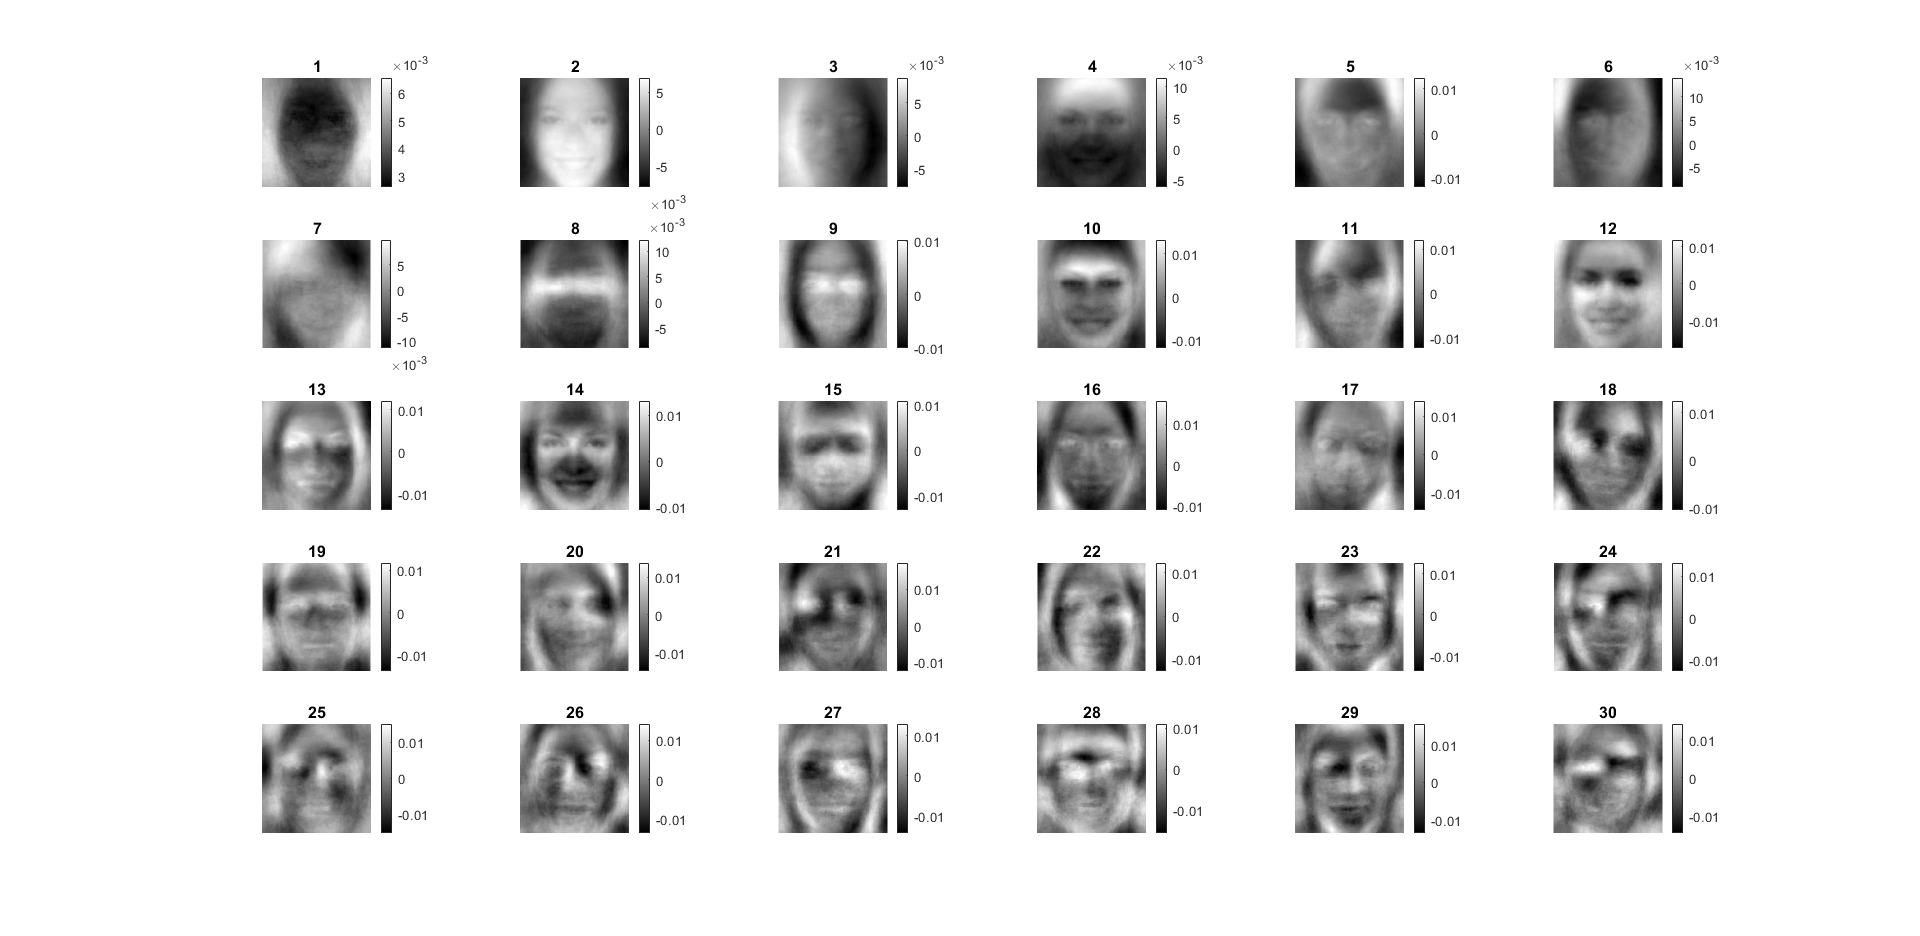
\includegraphics[width=\textwidth, height=\textheight, keepaspectratio]{eigenfaces1.png}
\end{figure}
\begin{figure}[htp]
	\centering
    \caption{Eigenfaces meno significative}
	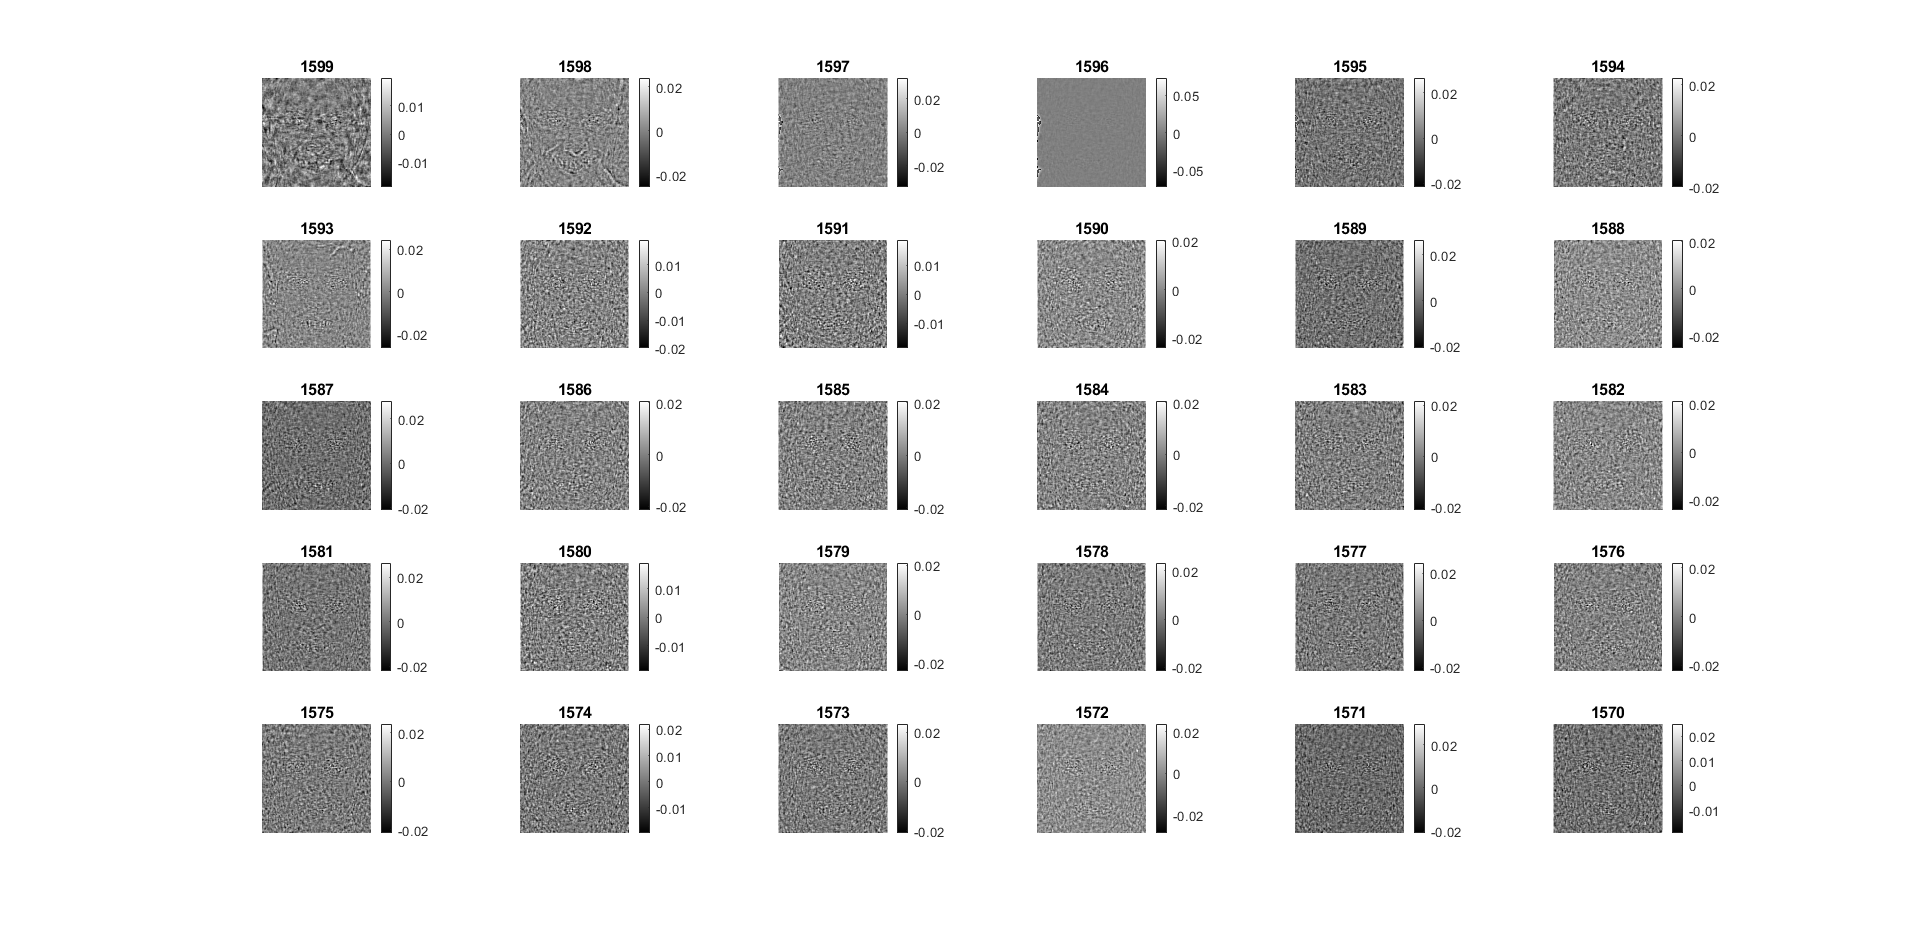
\includegraphics[width=\textwidth, height=\textheight, keepaspectratio]{eigenfaces2.png}
\end{figure}
\begin{figure}[htp]
	\centering
    \caption{Grafico dell'informazione modellata}
	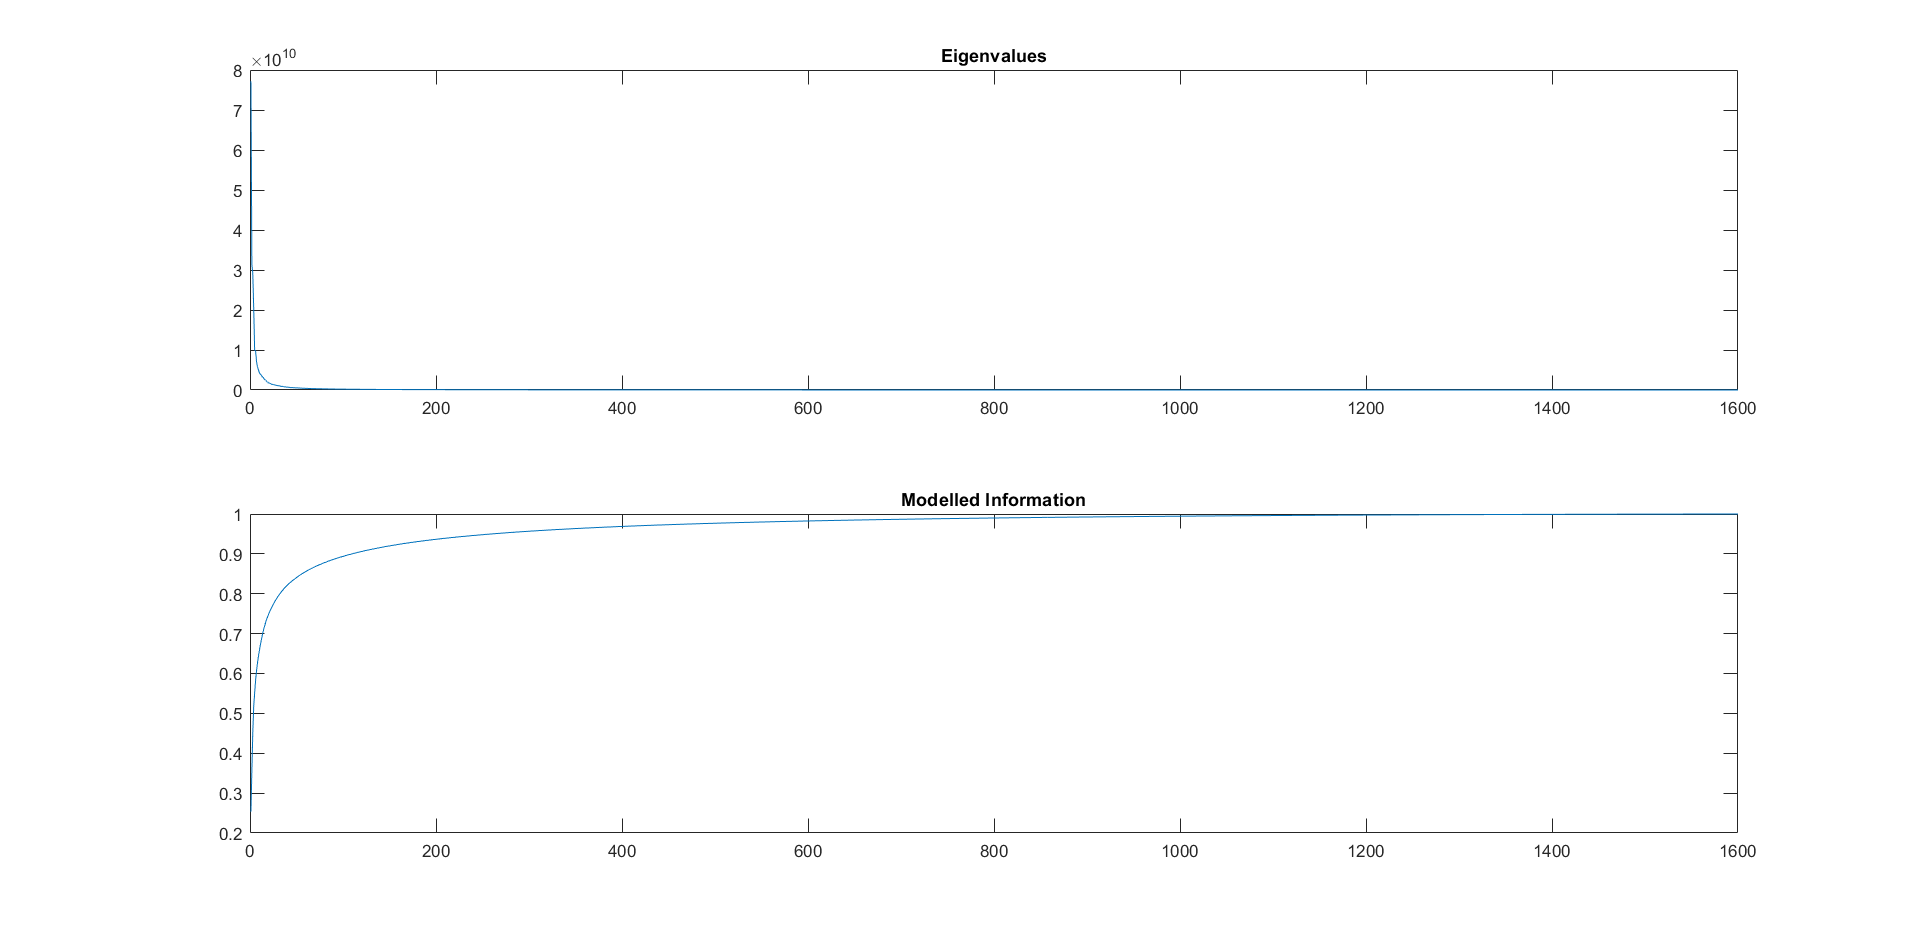
\includegraphics[width=\textwidth, height=\textheight, keepaspectratio]{informazione.png}
\end{figure}

\newpage
\section{Implementazione del classificatore}
Per implementare il classificatore sono state effettuate le seguenti operazioni:
\begin{enumerate}
    \item Si prende in input la matrice $(224 \cdot 224) \times 1600$ che rappresenta il train set (contiene i dati di 800 immagini di persone con la mascherina e 800 immagini di persone senza mascherina).
    \item Si prende in input la matrice $(224 \cdot 224) \times 800$ che rappresenta il validation set (contiene i dati di 400 immagini di persone con la mascherina e 400 immagini di persone senza mascherina).
    \item Si applica l'algoritmo delle eigenfaces sul train set e si esegue una proiezione in uno spazio $T$ dimensionale per ridurre il numero di features (le eigenfaces selezionate per la proiezione sono quelle più significative per un problema di face mask analysis).
    \item Si applica l'algoritmo delle eigenfaces e si esegue la stessa proiezione anche sul validation set.
    \item Si esegue la classificazione delle immagini nel validation set, tramite l'algoritmo KNN, e si valuta l'accuratezza.
\end{enumerate}

\newpage
\subsection{Algoritmo per le eigenfaces}
Se $A$ è una matrice di dimensione $N \times M$, allora la matrice di covarianza $S = A A'$ avrà dimensione $N \times N$. Il trucco che si può utilizzare per evitare il problema dell'\textit{overflow} consiste nel calcolare gli autovettori come $A' A$ (che ha una dimensione più gestibile pari a $M \times M$) in quanto nelle fasi successive, generalmente, non vengono usate più di 20-30 eigenfaces. I passi dell'algoritmo per le eigenfaces sono i seguenti:
\begin{enumerate}
    \item Sottrarre l'immagine media da ogni immagine presente nel dataset $A$.
    \item Calcolare gli $M$ autovalori di $A' A$ che corrispondono agli $M$ autovalori più grandi di $S = A A'$.
    \item Calcolare gli $M$ autovettori di $A' A$ formando la matrice $V$.
    \item Ottenere gli $M$ autovettori più grandi di $S = A A'$ calcolando $U = A V$.
\end{enumerate}
A questo punto è possibile ottenere i coefficienti di proiezione calcolando $\omega = U' A$.
\begin{minted}{matlab}
function [U,lambda] = eigen_training(A)
% Prende in input la matrice A risultante dalla sottrazione
% della media da ogni immagine presente.
% Applica l'algoritmo per le eigenfaces ma, a differenza di
% PCA, calcola la matrice di covarianza come A'A (invece di AA').
% Restituisce gli M autovalori di A'A (ovvero gli M autovalori
% più grandi di AA') e gli M autovettori più grandi di AA'
% calcolando AV.

M = size(A,2);
L = A'*A;

[V,valori] = eig(L);
valori = diag(valori);

[lambda,ind] = sort(valori,'descend');
V = V(:,ind);

U = A*V;

% Per avere vettori di norma 1 
for i=1:M
    U(:,i) = U(:,i)/norm(U(:,i));
end
\end{minted}

\subsection{Algoritmo KNN}
Il K-Nearest Neighbors (KNN) è un algoritmo di pattern recognition utilizzato per la classificazione di oggetti basandosi sulle caratteristiche degli oggetti vicini a quello considerato. Infatti, il KNN parte dall'idea che oggetti simili saranno vicini anche nello spazio delle features. Nella classificazione con KNN l'output è costituito dall'appartenenza di un oggetto ad una determinata classe: ogni oggetto viene assegnato alla classe che si presenta maggiormente tra i $K$ oggetti più vicini ad esso.
\begin{minted}{matlab}
function class = knnclassify(test,train,label,K)
% Dato un oggetto test e definito un valore intero positivo
% e non nullo K, si cercano i K oggetti più vicini a test
% nello spazio delle features rappresentato da train.
% Restituisce la classe che si presenta maggiormente tra i K
% oggetti selezionati.

num_c = size(train,1);

repe = repmat(test,num_c,1);
dist = sqrt(sum((repe-train).^2,2));

[~,ind] = sort(dist,'ascend');

label_ind = label(ind);

label_ind = label_ind(1:K);

num_classi = max(label);
for i = 1:num_classi
    win(i) = sum(double(label_ind == i));
end

[~,class] = max(win);
\end{minted}

\subsection{Selezione delle eigenfaces}
Per riuscire a selezionare le eigenfaces più significative per il problema si è deciso di far variare l'intervallo degli autovettori da usare per la proiezione in un range che comprende al massimo 30 autovettori, aumentando di 1 la lunghezza dell'intervallo ad ogni iterazione (fino ad un massimo di 15). Valutando l'accuratezza (vedi sezione \hyperref[acc]{\textit{Metriche statistiche}}) si può osservare che il valore più alto viene ottenuto quando si proietta in uno spazio i cui assi sono gli autovettori compresi tra il quarto e il quattordicesimo inclusi (vedi \hyperref[fig1]{\textit{Figura 1}}).

\`{E} ragionevole pensare che le prime tre eigenfaces si possono scartare perché rappresentano parti di volto o particolari illuminazioni i cui pesi non forniscono informazioni utili a verificare la presenza o meno di una mascherina. Guardando invece alle eigenfaces numero 4, 10, 12 e 14 si può notare che esse mostrano una zona intorno alla bocca con un'illuminazione differente da quella del resto del volto. Nelle rimanenti eigenfaces facenti parte dell'intervallo si può anche notare che ce ne sono alcune in cui il contorno della bocca non si vede proprio. Da tutto ciò si capisce l'importanza del peso di questi autovettori rispetto a quelli che sono stati scartati. Infatti, l'obiettivo di questo progetto non è quello di effettuare ricostruzioni, bensì di riuscire a creare uno spazio in cui risulti più semplice classificare immagini di persone che indossano o meno una mascherina. Inoltre, si vuole evitare il problema dell'\textit{overfitting}, ovvero non si vuole che il classificatore riesca a valutare perfettamente solo gli elementi del train set, per cui alla minima variazione dei valori delle features in un oggetto sconosciuto, la classificazione risulterebbe errata.
\begin{minted}{matlab}
load('train.mat', 'train_matrix');
train_matrix = double(train_matrix);
Mt = size(train_matrix,2);
train_label = reshape(repmat([1 2],Mt/2,1),Mt,1); % 2 classi da 800 immagini ciascuna

load('validation.mat', 'validation_matrix');
validation_matrix = double(validation_matrix);
Mv = size(validation_matrix,2);
validation_label = reshape(repmat([1 2],Mv/2,1),Mv,1); % 2 classi da 400 immagini ciascuna

% Algoritmo eigenfaces
media = mean(train_matrix,2);
A = train_matrix-repmat(media,1,Mt);
[U,lambda] = eigen_training(A);

acc_i = 1;
for passo = 1:15 % Considero varie dimensioni dell'intervallo (massimo 15)
    for j = 0:29 % Mi limito a 30 eigenfaces
        T_ind = 1+j:passo+j;
        omega_train = U(:,T_ind)'*A; % Proiezione del train set in uno spazio T dimensionale
        omega_validation = U(:,T_ind)'*(validation_matrix-repmat(media,1,Mv)); % Proiezione del validation set

        validation_i = 0;
        num_neigh = 5; % Numero di vicini per l'algoritmo KNN
        for i = 1:Mv
            validation_i = validation_i + 1;
            class = knnclassify(omega_validation(:,i)',omega_train',train_label,num_neigh);
            accuracy(validation_i) = class==validation_label(i);
        end

        fprintf('%i:%i accuracy = %f\n',1+j,passo+j,sum(accuracy)/size(accuracy,2));
        acc(acc_i) = sum(accuracy)/size(accuracy,2);
        acc_i = acc_i + 1;
    end
end

fprintf('%f\n',max(acc)); % Accuratezza più alta
\end{minted}

\section{Riconoscimento di nuove immagini}
Il sistema di riconoscimento effettua le seguenti operazioni:
\begin{enumerate}
    \item Si prende in input la matrice $(224 \cdot 224) \times 1600$ che rappresenta il train set\footnotemark[1] (contiene i dati di 800 immagini di persone con la mascherina e 800 immagini di persone senza mascherina).
    \item Si prende in input la matrice $(224 \cdot 224) \times 992$ che rappresenta il test set (contiene i dati di 483 immagini di persone con la mascherina e 509 immagini di persone senza mascherina).
    \item Si applica l'algoritmo delle eigenfaces sul train set e si esegue una proiezione in uno spazio $T$ dimensionale i cui assi sono gli autovettori selezionati durante la validazione.
    \item Si applica l'algoritmo delle eigenfaces e si esegue la stessa proiezione anche sul test set.
    \item Si esegue la classificazione delle immagini nel test set, tramite l'algoritmo KNN, e si costruisce la matrice di confusione per valutare le misure di accuratezza.
\end{enumerate}

\footnotetext[1]{Nel \href{https://www.kaggle.com/ashishjangra27/face-mask-12k-images-dataset}{dataset} ci sono 10000 train images; ne sono state usate 1600 per questioni di complessità spaziale}

\subsection{Matrice di confusione}
Per un problema di classificazione a $C$ classi, la matrice di confusione ha dimensione $C \times C$. Quindi, nel caso in esame sarà nella forma:
\begin{center}
\begin{tabular}{ccc}
    \toprule
    & \textit{Con mascherina} & \textit{Senza mascherina} \\
    
    \midrule
    \textit{Con mascherina} & TP & FN \\
    
    \midrule
    \textit{Senza mascherina} & FP & TN \\

    \bottomrule
\end{tabular}
\end{center}
Le righe indicano la classe reale (ground truth), mentre le colonne indicano la classe riconosciuta (risultato del classificatore). Inoltre:
\begin{itemize}
    \item TP identifica i veri positivi, ossia quegli oggetti appartenenti ad una determinata classe che vengono correttamente riconosciuti come membri di quella classe (successo).
    \item FP identifica i falsi positivi, ossia quegli oggetti che vengono riconosciuti come appartenenti ad una determinata classe ma che in realtà non vi appartengono (falso allarme, sovrastima).
    \item FN identifica i falsi negativi, ossia tutti quegli oggetti che appartengono ad una classe ma che non vengono riconosciuti come tali (insuccesso, sottostima).
    \item TN identifica i veri negativi, ossia tutti quegli oggetti che non appartengono ad una classe e che vengono riconosciuti come tali (rigettato correttamente).
\end{itemize}

\subsection{Metriche statistiche}
\label{acc}
Di seguito vengono date le definizioni di varie metriche statistiche che si possono ricavare dalla matrice di confusione.
\paragraph{True Positive Rate (TPR).} Misura il tasso di positivi correttamente individuati, ossia la probabilità che gli oggetti affetti da qualche condizione siano correttamente identificati come affetti da quella condizione. Il TPR viene anche chiamato sensitività.
\[ \frac{TP}{TP+FN} \]
\paragraph{True Negative Rate (TNR).} Misura il tasso di negativi correttamente individuati, ossia la probabilità che oggetti non affetti da una particolare condizione siano correttamente identificati come non affetti da quella condizione. Il TNR viene anche chiamato specificità.
\[ \frac{TN}{TN+FP} \]
\paragraph{False Positive Rate (FPR).} Misura il tasso di negativi che producono risultati positivi, ossia la probabilità condizionata di ottenere un risultato positivo partendo dal fatto che la condizione cercata non era presente.
\[ \frac{FP}{FP+TN} \]
\paragraph{False Negative Rate (FNR).} Misura il tasso di positivi che producono risultati negativi, ossia la probabilità condizionata di ottenere un risultato negativo partendo dal fatto che la condizione cercata era presente.
\[ \frac{FN}{FN+TP} \]
\paragraph{Precisione.} Nell'ambito della classificazione, la precisione di una classe è data dal numero di oggetti etichettati correttamente come appartenenti a quella classe diviso il numero totale di elementi etichettati come appartenenti a quella classe.
\[ \frac{TP}{TP+FP} \]
\paragraph{Accuratezza.} Misura il grado di vicinanza fra i dati osservati e quelli attesi. Per un classificatore binario, l'accuratezza indica quanto correttamente esso riesce a riconoscere gli oggetti come appartenenti ad una classe oppure all'altra. La metrica assume quindi valori vicini a 1 quanto più i falsi positivi e i falsi negativi assumono valori vicini a 0, cioè quando il classificatore riesce a distinguere bene se un oggetto è membro di una classe oppure no.
\[ \frac{TP+TN}{(TP+FP)+(TN+FN)} \]

\subsection{Risultati e considerazioni finali}
Al termine della fase di testing è stata ottenuta la seguente matrice di confusione:
\begin{center}
\begin{tabular}{cccc}
    \toprule
    & \textit{Con mascherina} & \textit{Senza mascherina} & \textbf{TOTALE} \\
    
    \midrule
    \textit{Con mascherina} & 308 & 175 & \textbf{483} \\
    
    \midrule
    \textit{Senza mascherina} & 29 & 480 & \textbf{509} \\
    
    \bottomrule
\end{tabular}
\end{center}
Di seguito i risultati del calcolo delle metriche statistiche presentate nella sezione precedente:
\begin{center}
\begin{tabular}{cc}
    \toprule
    \textit{Metrica} & \textit{Risultato} \\
    
    \midrule
    TPR & 0.637681 \\
    \midrule
    TNR & 0.943026 \\
    \midrule
    FPR & 0.056974 \\
    \midrule
    FNR & 0.362319 \\
    \midrule
    Precisione & 0.913947 \\
    \midrule
    Accuratezza & 0.794355 \\
    
    \bottomrule
\end{tabular}
\end{center}
Su tali valori è possibile fare alcune considerazioni:
\begin{itemize}
    \item La probabilità che una persona ``con'' sia classificata come ``con'' è all'incirca del 64 \%, indicando una certa tendenza a creare falsi ``senza''.
    \item La probabilità che una persona ``senza'' sia classificata come ``senza'' è all'incirca del 94 \%, indicando una bassa tendenza a creare falsi ``con''.
    \item Il valore di precisione della classe ``con'' conferma il punto precedente.
    \item Il valore di accuratezza è paragonabile a quello ottenuto nella fase di validazione confermando la bontà della scelta degli autovettori su cui è stata fatta la proiezione.
\end{itemize}
\begin{minted}{matlab}
load('train.mat', 'train_matrix');
train_matrix = double(train_matrix);
M = size(train_matrix,2);
train_label = reshape(repmat([1 2],M/2,1),M,1); % 2 classi da 800 immagini ciascuna

load('test.mat', 'test_matrix');
test_matrix = double(test_matrix);
Mt = size(test_matrix,2);
test_label = ones(Mt,1); % 1a classe da 483 immagini
test_label(484:end) = test_label(484:end)*2; % 2a classe da 509 immagini

% Algoritmo eigenfaces
media = mean(train_matrix,2);
A = train_matrix-repmat(media,1,M);
[U,lambda] = eigen_training(A);

% Proiezioni nello spazio T dimensionale
T_ind = 4:14;  % Indici degli autovettori (dalla fase di validazione)
omega_train = U(:,T_ind)'*A; % Proiezione del train set
omega_test = U(:,T_ind)'*(test_matrix-repmat(media,1,Mt)); % Proiezione del test set

confmat = zeros(2,2); % Matrice di confusione

num_neigh = 5; % Numero di vicini per il KNN
for i = 1:Mt
    class = knnclassify(omega_test(:,i)',omega_train',train_label,num_neigh);
    confmat(test_label(i),class) = confmat(test_label(i),class)+1;  
end

% Metriche statistiche
confmat
fprintf('Accuratezza = %f\n',(confmat(1,1)+confmat(2,2))/sum(confmat,'all'));
fprintf('Precisione = %f\n',confmat(1,1)/(confmat(1,1)+confmat(2,1)));
fprintf('TPR = %f\n',confmat(1,1)/(confmat(1,1)+confmat(1,2)));
fprintf('TNR = %f\n',confmat(2,2)/(confmat(2,2)+confmat(2,1)));
fprintf('FPR = %f\n',confmat(2,1)/(confmat(2,1)+confmat(2,2)));
fprintf('FNR = %f\n',confmat(1,2)/(confmat(1,2)+confmat(1,1)));
\end{minted}

\end{document}